\subsection{Transaction}
\label{sec:transaction}

Trong kiến trúc Microservices và Polyglot Persistence của hệ thống E-commerce, việc đảm bảo tính toàn vẹn dữ liệu khi thao tác trên nhiều loại cơ sở dữ liệu khác nhau là một thách thức lớn. Vì vậy mục này sẽ phân tích sâu cơ chế Transaction trên hai hệ quản trị cơ sở dữ liệu được nhóm sử dụng là \textbf{PostgreSQL} (cho dữ liệu nghiệp vụ cốt lõi) và \textbf{MongoDB} (cho dữ liệu sản phẩm và logs), đồng thời so sánh hiệu năng và cách ứng dụng thực tế.

\subsubsection{Giới thiệu chung và Bài toán E-commerce}
Transaction (Giao dịch) là một chuỗi các thao tác truy xuất hoặc cập nhật dữ liệu được thực hiện như một đơn vị công việc logic duy nhất. Nguyên tắc cốt lõi là \textit{"all-or-nothing"} - hoặc toàn bộ thành công (Commit), hoặc toàn bộ bị hủy bỏ (Rollback).\medskip

Trong ngữ cảnh ứng dụng E-commerce Platform của nhóm, Transaction đóng vai trò vô cùng quan trọng trong quy trình "Đặt hàng" (Order Placement). Đối với một giao dịch đặt hàng hợp lệ, nhóm đề xuất phải đảm bảo các bước sau diễn ra đồng thời:

\begin{enumerate}
    \item Kiểm tra và trừ số lượng tồn kho trong bảng (PostgreSQL).
    \item Tạo bản ghi đơn hàng mới trong bảng(PostgreSQL).
    \item Ghi log hành vi người dùng (MongoDB).
\end{enumerate}

Nếu bước trừ kho thành công nhưng bước tạo đơn hàng thất bại, dữ liệu sẽ bị sai lệch, dẫn đến mất mát tài sản. Do đó, hệ thống tuân thủ chặt chẽ 4 tính chất ACID: \textbf{Atomicity, Consistency, Isolation, Durability}.

\begin{itemize}[label=$\circ$]
    \item \textbf{Tính nguyên tử (Atomicity):} Đảm bảo transaction là bất khả phân.
    \item \textbf{Tính nhất quán (Consistency):} Dữ liệu phải chuyển từ trạng thái hợp lệ này sang trạng thái hợp lệ khác.
    \item \textbf{Tính độc lập (Isolation):} Các transaction chạy song song không được ảnh hưởng lẫn nhau.
    \item \textbf{Tính bền vững (Durability):} Dữ liệu đã commit sẽ được lưu trữ vĩnh viễn.
\end{itemize}

\subsubsection{Transaction trong PostgreSQL}

PostgreSQL là hệ quản trị cơ sở dữ liệu quan hệ (RDBMS) tuân thủ nghiêm ngặt chuẩn ACID, sử dụng cơ chế Write-Ahead Logging - WAL để đảm bảo tính bền vững.

\paragraph{Vòng đời và Quản lý Transaction}

Trong PostgreSQL, một transaction trải qua các trạng thái từ khi kích hoạt (Active) đến khi hoàn tất (Committed) hoặc thất bại (Aborted).

\begin{figure}[H]
    \centering
    \begin{tikzpicture}[
        node distance=2cm,
        startstop/.style={rectangle, rounded corners, minimum width=3cm, minimum height=1cm, text centered, draw=black, fill=blue!10},
        process/.style={rectangle, minimum width=3cm, minimum height=1cm, text centered, draw=black, fill=orange!10},
        decision/.style={diamond, aspect=2, minimum width=3cm, minimum height=1cm, text centered, draw=black, fill=green!10},
        arrow/.style={thick,->,>=stealth}
    ]
    \node (active) [startstop] {Active};
    \node (partial) [process, right=of active] {Partially Committed};
    \node (committed) [startstop, right=of partial] {Committed};
    \node (failed) [process, below=of partial] {Failed};
    \node (aborted) [startstop, below=of failed] {Aborted};

    \draw [arrow] (active) -- node[anchor=south] {Read/Write} (partial);
    \draw [arrow] (partial) -- node[anchor=south] {Commit} (committed);
    \draw [arrow] (active) -- node[anchor=east] {Error} (failed);
    \draw [arrow] (partial) -- node[anchor=east] {Error} (failed);
    \draw [arrow] (failed) -- node[anchor=east] {Rollback} (aborted);
    \end{tikzpicture}
    \caption{Sơ đồ chuyển đổi trạng thái Transaction trong PostgreSQL}
    \label{fig:transaction_states}
\end{figure}

Một vòng đời tiêu chuẩn trong PostgreSQL sẽ bao gồm:
\begin{itemize}[label=$\circ$]
    \item \textbf{Active:} Giao dịch đang thực thi các lệnh SQL.
    \item \textbf{Partially Committed:} Các thao tác đã hoàn tất trong bộ nhớ đệm, chờ ghi vào nhật ký hệ thống (Logs).
    \item \textbf{Committed:} Giao dịch thành công, dữ liệu an toàn.
    \item \textbf{Aborted/Rolled Back:} Giao dịch thất bại, hệ thống hoàn tác về trạng thái cũ.
\end{itemize}

Ví dụ thực tế trong một module \texttt{Order Service}: Sử dụng \texttt{BEGIN} để bắt đầu và \texttt{COMMIT} để kết thúc. 
\begin{verbatim}
BEGIN;
-- 1. Trừ tồn kho (Sử dụng khóa bi quan để tránh Race Condition)
UPDATE inventory SET quantity = quantity - 1 
WHERE product_id = 101 AND quantity > 0;
-- 2. Tạo đơn hàng
INSERT INTO orders(user_id, total_price) VALUES (5, 12000000);
-- 3. Nếu mọi thứ ổn
COMMIT;
\end{verbatim}

\paragraph{Cơ chế MVCC và Isolation Levels}
Khác với các RDBMS truyền thống sử dụng khóa (Locking) gây tắc nghẽn, PostgreSQL sử dụng \textbf{MVCC (Multi-Version Concurrency Control)}.
\begin{itemize}[label=$\circ$]
    \item Mỗi transaction nhìn thấy một bản chụp (snapshot) dữ liệu tại thời điểm nó bắt đầu.
    \item Readers never block Writers và Writers never block Readers.
\end{itemize}

PostgreSQL hỗ trợ 3 mức cô lập chính (mặc định là Read Committed):
\begin{itemize}[label=$\circ$]
    \item \textbf{Read Committed:} Transaction chỉ nhìn thấy dữ liệu đã được commit.
    \item \textbf{Repeatable Read:} Đảm bảo nhất quán dữ liệu trong suốt quá trình transaction diễn ra (Sử dụng cho báo cáo thống kê doanh thu).
    \item \textbf{Serializable:} Mức cao nhất, giả lập thực thi tuần tự để tránh mọi xung đột (Phantom Read) \cite{postgresql_docs}.
\end{itemize}

\paragraph{Giao thức Two-Phase Commit (2PC)}
Khi hệ thống cần đồng bộ trạng thái giữa PostgreSQL (Lưu đơn hàng) và một dịch vụ thanh toán bên ngoài (Payment Gateway), giao thức 2PC được sử dụng để đảm bảo tính nguyên tử phân tán. PostgreSQL hỗ trợ điều này qua lệnh \texttt{PREPARE TRANSACTION}.

\begin{figure}[H]
    \centering
    \begin{tikzpicture}[
        node distance=3.5cm, % Tăng khoảng cách để sơ đồ rộng hơn
        auto,
        thick,
        % Tăng chiều rộng ô actor lên 2.8cm cho thoáng
        actor/.style={rectangle, draw=black, fill=blue!10, thick, minimum width=2.8cm, minimum height=1cm, align=center, font=\small}, 
        msg/.style={->, >=stealth, thick},
        timeline/.style={dashed, thick, gray}
    ]
        % Khai báo các Node
        \node[actor] (coord) {Coordinator};
        \node[actor, right=of coord] (part1) {PostgreSQL};
        \node[actor, right=of part1] (part2) {Payment Svc};

        % Vẽ đường timeline
        \draw[timeline] (coord.south) -- ++(0,-7.5) coordinate (coord_end); % Tăng độ dài timeline xuống chút
        \draw[timeline] (part1.south) -- ++(0,-7.5) coordinate (part1_end);
        \draw[timeline] (part2.south) -- ++(0,-7.5) coordinate (part2_end);

        % --- PHASE 1 ---
        \node[anchor=east, font=\bfseries\small] at ($(coord.south) + (-0.2,-1)$) {Phase 1};

        % Prepare Request
        \draw[msg, blue] ($(coord.south) + (0,-1)$) -- node[above, font=\footnotesize] {Prepare?} ($(part1.south) + (0,-1)$);
        \draw[msg, blue] ($(coord.south) + (0,-1.5)$) -- node[above, font=\footnotesize, sloped] {Prepare?} ($(part2.south) + (0,-1.5)$);

        % Vote Response
        \draw[msg, dashed, blue] ($(part1.south) + (0,-2.5)$) -- node[above, font=\footnotesize] {Vote Yes} ($(coord.south) + (0,-2.5)$);
        \draw[msg, dashed, blue] ($(part2.south) + (0,-3.0)$) -- node[above, font=\footnotesize, sloped] {Vote Yes} ($(coord.south) + (0,-3.0)$);

        % --- PHASE 2 ---
        \node[anchor=east, font=\bfseries\small] at ($(coord.south) + (-0.2,-4.5)$) {Phase 2};

        % Commit Command
        \draw[msg, red] ($(coord.south) + (0,-4.5)$) -- node[above, font=\footnotesize] {Commit!} ($(part1.south) + (0,-4.5)$);
        \draw[msg, red] ($(coord.south) + (0,-5.0)$) -- node[above, font=\footnotesize, sloped] {Commit!} ($(part2.south) + (0,-5.0)$);

        % Ack Response
        \draw[msg, dashed, red] ($(part1.south) + (0,-6.0)$) -- node[above, font=\footnotesize] {Ack} ($(coord.south) + (0,-6.0)$);
        \draw[msg, dashed, red] ($(part2.south) + (0,-6.5)$) -- node[above, font=\footnotesize, sloped] {Ack} ($(coord.south) + (0,-6.5)$);

    \end{tikzpicture}
    \caption{Mô phỏng Two-Phase Commit giữa PostgreSQL và Payment Service}
    \label{fig:2pc_protocol}
\end{figure}

\subsubsection{Transaction trong MongoDB}

Trước phiên bản 4.0, MongoDB chỉ đảm bảo tính nguyên tử trên một document đơn lẻ. Tuy nhiên, với sự ra đời của \textbf{Multi-document ACID Transactions} (v4.0+), MongoDB đã tiệm cận khả năng của RDBMS, cho phép cập nhật nguyên tử trên nhiều collection và database \cite{mongodb_transactions}.

\paragraph{Mô hình Eventual Consistency và Replica Set}
Mặc dù đã hỗ trợ ACID, nhưng trong mô hình phân tán (Sharding/Replication) mặc định, MongoDB ưu tiên tính sẵn sàng (Availability). Khi dữ liệu được ghi vào node Primary, cần một khoảng thời gian để đồng bộ sang các node Secondary.

\begin{figure}[H]
    \centering
    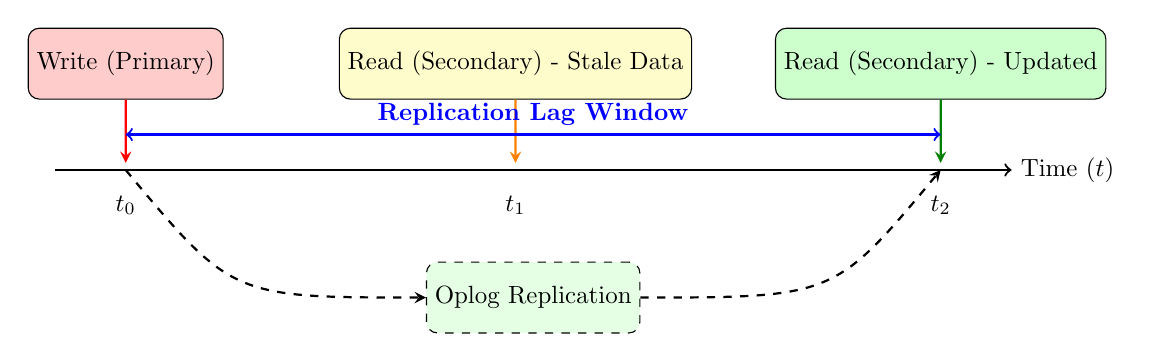
\begin{tikzpicture}[
        node distance=2cm,
        scale=0.9, transform shape,
        process/.style={rectangle, draw=black, fill=blue!10, rounded corners, minimum width=2.5cm, minimum height=1cm},
        arrow/.style={->, >=stealth, thick},
        timeline/.style={->, thick}
    ]
    % Time Axis
    \draw[timeline] (-2.5,0) -- (11,0) node[right] {Time ($t$)};
    % Events
    \node (write) at (-1.5, 1.5) [process, fill=red!20] {Write (Primary)};
    \draw[arrow, red] (write) -- (-1.5,0.1);
    \node at (-1.5, -0.5) {$t_0$};

    \node (read_fail) at (4, 1.5) [process, fill=yellow!20] {Read (Secondary) - Stale Data};
    \draw[arrow, orange] (read_fail) -- (4,0.1);
    \node at (4, -0.5) {$t_1$};

    \node (sync) at (4.25, -1.8) [process, fill=green!10, dashed] {Oplog Replication};
    \draw[arrow, dashed] (-1.5, 0) .. controls (0, -1.8) .. (sync.west);
    \draw[arrow, dashed] (sync.east) .. controls (8.5, -1.8) .. (10, 0);

    \node (read_success) at (10, 1.5) [process, fill=green!20] {Read (Secondary) - Updated};
    \draw[arrow, green!50!black] (read_success) -- (10,0.1);
    \node at (10, -0.5) {$t_2$};

    % Annotations
    \draw[<->, thick, blue] (-1.5,0.5) -- (10,0.5) node[midway, above] {\textbf{Replication Lag Window}};
    \end{tikzpicture}
    \caption{Cơ chế Eventual Consistency trong MongoDB Replica Set: Dữ liệu cần thời gian để Oplog đồng bộ từ Primary sang Secondary.}
    \label{fig:eventual_consistency}
\end{figure}

\paragraph{Single-Document vs. Multi-Document Transaction}
Trong ứng dụng E-commerce, nhóm ưu tiên thiết kế dữ liệu dạng Embedded (Nhúng) để tận dụng Single-Document Atomicity. Ví dụ: Lưu danh sách đánh giá (Reviews) ngay bên trong document Product. Điều này giúp thao tác ghi nhanh hơn và không cần mở transaction phức tạp.\medskip

Tuy nhiên, với các nghiệp vụ cần cập nhật nhiều bảng (ví dụ: chuyển trạng thái Flash Sale cho nhiều sản phẩm), nhóm ưu tiên sử dụng Multi-Document Transaction với cơ chế Snapshot Isolation của WiredTiger engine.

\begin{figure}[H]
    \centering
    \begin{tikzpicture}[
        node distance=1cm,
        doc/.style={rectangle, draw=black, fill=white, drop shadow, minimum width=3.5cm, minimum height=4cm, align=left, font=\small\ttfamily},
        box/.style={rectangle, draw=red, dashed, thick, rounded corners, inner sep=10pt},
        arrow/.style={->, >=stealth, ultra thick, blue}
    ]
    \node[doc] (single) at (0,0) {
        \textbf{\{JSON: Product\}}\\
        \_id: 101\\
        name: "Laptop"\\
        \textbf{reviews: [}\\
        \ \ \{user: "A", rate: 5\},\\
        \ \ \{user: "B", rate: 4\}\\
        \textbf{]}\\
        price: 2000
    };
    \node[above=1.75cm of single, font=\bfseries] {Embedded Design (Atomic)};
    \draw[arrow] (-5, 0) -- node[above, font=\bfseries, text=black] {Single Write} (single.west);

    \node[doc, minimum height=1.5cm] (order) at (7, 1.5) {
        \textbf{\{Coll: Products\}}\\
        \_id: 101, stock: 49
    };
    \node[doc, minimum height=1.5cm] (stock) at (7, -1.5) {
        \textbf{\{Coll: Logs\}}\\
        action: "SALE\_UPDATE"
    };

    \node[above=1.5cm of order, font=\bfseries] {Normalized Design (Multi-Doc)};
    \node[draw=green!50!black, thick, dashed, fit=(order) (stock), label=above:\textcolor{green!50!black}{\textbf{ACID Transaction Scope}}] (trans) {};

    \draw[arrow] (11.5, 0) -- node[above, font=\bfseries, text=black] {Session Start} (trans.east);
    \draw[->, thick] (trans.center) -- (order.south);
    \draw[->, thick] (trans.center) -- (stock.north);
    \end{tikzpicture}
    \caption{Chiến lược thiết kế: Ưu tiên Embedded (trái) để giảm tải Transaction, chỉ dùng Transaction (phải) khi bắt buộc.}
    \label{fig:single_vs_multi_doc}
\end{figure}

\subsubsection{So sánh và Kết luận lựa chọn}

Dựa trên thực nghiệm, nhóm đúc kết bảng so sánh chi tiết giữa hai hệ quản trị cho bài toán E-commerce:

\begin{table}[H]
\centering
\renewcommand{\arraystretch}{1.4}
\begin{tabularx}{\textwidth}{|l|X|X|}
\hline
\textbf{Tiêu chí} & \textbf{PostgreSQL} & \textbf{MongoDB} \\ \hline
\textbf{Cơ chế lõi} & \textbf{MVCC}: Tối ưu cho môi trường nhiều người đọc/ghi đồng thời mà không lock bảng. & \textbf{WiredTiger Snapshot}: Sử dụng cơ chế copy-on-write để quản lý các phiên bản document. \\ \hline
\textbf{Phạm vi Transaction} & \textbf{Global}: Transaction có thể bao trùm toàn bộ các bảng trong database, hỗ trợ ràng buộc khóa ngoại (FK) chặt chẽ. & \textbf{Flexible}: Transaction đa tài liệu hoạt động trên Replica Set. Tuy nhiên, giới hạn transaction time (mặc định 60s) và kích thước Oplog. \\ \hline
\textbf{Hiệu năng} & Ổn định cho các giao dịch phức tạp (Complex Join + Write). Tuy nhiên, bảng lớn có thể gặp vấn đề về VACUUM (dọn dẹp dữ liệu cũ). & Tốc độ ghi cực nhanh với Single-document. Transaction đa tài liệu làm giảm hiệu năng khoảng 2-4 lần so với ghi thường do overhead đồng bộ. \\ \hline
\textbf{Ứng dụng trong đồ án} & Quản lý \textbf{Users, Orders, Inventory, Payments} (Yêu cầu ACID tuyệt đối). & Quản lý \textbf{Product Catalog, Reviews, Logs} (Cần linh hoạt schema, chấp nhận Eventual Consistency ở một số tác vụ đọc). \\ \hline
\end{tabularx}
\caption{So sánh đặc tính Transaction giữa PostgreSQL và MongoDB trong dự án}
\label{tab:sql_nosql_trans}
\end{table}

\textbf{Kết luận:} Việc kết hợp PostgreSQL cho dữ liệu giao dịch cốt lõi và MongoDB cho dữ liệu phi cấu trúc giúp hệ thống đạt được sự cân bằng giữa tính an toàn (Safety) và hiệu năng (Performance), đồng thời đáp ứng tốt yêu cầu Bonus của đề tài.